\documentclass[11pt,a4paper]{article}

\usepackage[utf8]{inputenc}
\usepackage[T1]{fontenc}
\usepackage{lmodern}
\usepackage{amsmath,amssymb}
\usepackage[margin=1in]{geometry}
\usepackage{graphicx}
\usepackage{booktabs}
\usepackage{array}
\usepackage{xcolor}
\usepackage{listings}
\usepackage{caption}
\usepackage{siunitx}
\usepackage[colorlinks=true,linkcolor=blue,urlcolor=blue]{hyperref}

\definecolor{codebg}{gray}{0.96}
\definecolor{codeframe}{gray}{0.78}
\definecolor{codecomment}{rgb}{0.0,0.5,0.0}
\lstset{
  basicstyle=\ttfamily\small, breaklines=true, frame=single, framerule=0.6pt,
  rulecolor=\color{codeframe}, backgroundcolor=\color{codebg},
  commentstyle=\color{codecomment}, columns=flexible,
  xleftmargin=1em, xrightmargin=1em, aboveskip=1em, belowskip=1em
}

% best / warn highlights for table cells
\newcommand{\best}[1]{\textbf{#1}}
\newcommand{\warn}[1]{\textcolor{red!75!black}{#1}}
\newcommand{\dd}{\textendash\textendash}

\title{\textbf{Choosing the sampler for the flattened tropical integrand}\\[2pt]
\large Plain Monte Carlo vs.\ quasi--Monte Carlo vs.\ CUBA, applied
\emph{after} tropical decomposition and flattening}
\author{Tropical Monte Carlo v2 --- \texttt{TEST/} benchmark}
\date{\today}

\begin{document}
\maketitle

\begin{abstract}
The Tropical Monte Carlo v2 pipeline reduces a convergent generalized Euler
integral to a sum of per-sector integrals that are bounded and $O(1)$ on the
unit cube $[0,1]^n$, then evaluates each with plain uniform Monte Carlo. This
report asks whether, \emph{given those already-flattened sectors}, it is faster
to use quasi--Monte Carlo (QMC) or an adaptive library such as CUBA. Across
15~higher-dimensional convergent integrands ($n=2\ldots 8$, four families, each
with an exact closed form), feeding the \emph{identical} flattened sector
functions to six samplers, the conclusion is: plain MC is the weakest option;
\textbf{CUBA-Vegas} (Sobol-seeded adaptive importance sampling) is the overall
winner, with the best accuracy-per-evaluation in every case and a convergence
rate that does not degrade with dimension; randomized \textbf{Sobol QMC} is the
best dependency-light upgrade over MC; \textbf{Cuhre} is unbeatable only when
flattening leaves a smooth integrand (integer effective exponents), and
\textbf{Divonne} can return confidently wrong answers and should be avoided.
The key mechanism is that flattening guarantees $O(1)$ \emph{magnitude} but not
\emph{smoothness}: a non-unit effective exponent injects a fractional power
(e.g.\ $\sqrt{y}$) at a cube face, which breaks polynomial cubature.
Quantitatively, Vegas reaches a given accuracy with ${\sim}150\times$ (at
$10^{-3}$) to ${\sim}2300\times$ (at $10^{-4}$) fewer evaluations than plain MC,
the advantage growing as the target tightens. Finally, the tropical
preprocessing remains essential: run head-to-head against Vegas on the
\emph{raw} integrand, the flattened decomposition is more accurate at fewer
evaluations --- by ${\sim}340\times$ on an integrand with a genuine $x^{-1/2}$
singularity.
\end{abstract}

%=============================================================================
\section{Background}
After Steps 1--4 of the algorithm, the integral is the exact sum
\begin{equation}\label{eq:master}
I=\sum_\sigma \frac{|\det M_\sigma|}{\prod_j a^\sigma_j}
  \int_{[0,1]^n}\!\! d^n y'\;\prod_k Q^\sigma_k\!\big({y'}^{1/a^\sigma}\big)^{B_k},
\end{equation}
where each summand is, by design, ``a smooth, bounded, $O(1)$ function on the
unit cube.'' The shipped C++ samples each sector with \texttt{std::mt19937\_64}
and Welford statistics. This report keeps the left-hand side of
\eqref{eq:master} fixed and varies only how the right-hand side integrals are
estimated. (The package's existing CUBA cross-checks integrate the
\emph{original, un-decomposed} integrand via a $x_i=t_i/(1-t_i)$
compactification; here CUBA and QMC act on the \emph{post-flattening} sectors.)

%=============================================================================
\section{Experimental design}

\subsection{Test integrands}
All convergent, numeric, parameter-free, with an analytic reference, and
generated by the real pipeline (\texttt{ProcessSector} /
\texttt{GenerateCppMonteCarlo}).

\begin{center}\small
\begin{tabular}{@{}llccl@{}}
\toprule
Family & $\displaystyle\int_{[0,\infty)^n}\!\!\prod_i x_i^{A_i}\,P^{B}\,d^nx$ & $n$ & sectors & exact \\
\midrule
A simplex      & $P=1+\sum_i x_i,\ A_i=0,\ B=-(n{+}2)$        & 2\dots8 & $n{+}1$ & $1/(n{+}1)!$ \\
Af frac.\ simp.& $P=1+\sum_i x_i,\ A_i=-\tfrac12,\ B=-(n{+}1)$ & 2,4,6   & $n{+}1$ & $\pi^{n/2}\Gamma(\tfrac n2{+}1)/n!$ \\
B quadratic    & $P=1+\sum_i x_i^2,\ A_i=0,\ B=-(n{+}1)$       & 4,6     & $n{+}1$ & $2^{-n}\pi^{n/2}\Gamma(\tfrac n2{+}1)/n!$ \\
D product      & $P=\prod_i(1{+}x_i),\ A_i=0,\ B=-2$           & 3,4,5   & $2^{n}$ & $1$ \\
\bottomrule
\end{tabular}
\end{center}

\noindent Family~A is the dimension-scaling spine. Af adds genuine $x^{-1/2}$
edge singularities that exercise the flattening. B gives a different integrand
shape. D has a hypercube Newton polytope, hence $2^n$ sectors, stressing sector
count and per-call library overhead.

\subsection{Methods (all single-threaded, identical integrands)}
\begin{center}\small
\begin{tabular}{@{}ll@{}}
\toprule
\textbf{MC}      & plain pseudo-random uniform MC (\texttt{mt19937\_64}) --- \emph{the shipped pipeline} \\
\textbf{QMC}     & randomized QMC: Boost \texttt{sobol} (Joe--Kuo) + 16 Cranley--Patterson random shifts \\
\textbf{VEGAS}   & CUBA Vegas --- adaptive importance sampling on Sobol points (\texttt{seed=0}) \\
\textbf{SUAVE}   & CUBA Suave --- subregion-adaptive importance sampling \\
\textbf{DIVONNE} & CUBA Divonne --- stratified sampling / region splitting \\
\textbf{CUHRE}   & CUBA Cuhre --- deterministic globally-adaptive polynomial cubature \\
\bottomrule
\end{tabular}
\end{center}

\subsection{Metric and fairness}
For each method I sweep a per-sector budget $N\in\{10^3,\dots,10^6\}$, sum the
sectors, and compute the \emph{true} relative error against the analytic
reference. Budgets mean samples per sector (MC/QMC) and \texttt{maxeval} per
sector (CUBA). Everything is single-threaded (\texttt{cubacores(0,0)}). A QMC
canary (integrating $e^{\sum_i y_i}$, exact $(e-1)^n$) verifies the Sobol
generator delivers low-discrepancy convergence.

%=============================================================================
\section{Decomposition correctness}
At the top budget, five independent samplers agree with the exact value in
every case; the lone outlier is Divonne. For the hardest case
\texttt{A\_simplex\_n8} (exact $=1/9!=\num{2.75573e-6}$):

\begin{center}\small
\begin{tabular}{@{}lcc@{}}
\toprule
method & estimate & rel.\ error \\
\midrule
MC      & \num{2.72035e-6} & \num{1.28e-2} \\
QMC     & \num{2.77275e-6} & \num{6.18e-3} \\
\best{VEGAS}   & \best{\num{2.75743e-6}} & \best{\num{6.18e-4}} \\
SUAVE   & \num{2.73838e-6} & \num{6.30e-3} \\
DIVONNE & \num{2.15019e-6} & \warn{\num{2.20e-1}} \\
CUHRE   & \num{2.74215e-6} & \num{4.93e-3} \\
\bottomrule
\end{tabular}
\end{center}
Five methods bracket the exact value, so the tropical decomposition is correct;
Divonne's $22\%$ miss is a \emph{method} failure. No NaN/Inf occurred in the
769-row dataset.

%=============================================================================
\section{The QMC generator works (canary)}
Integrating the smooth $e^{\sum y_i}$, MC hugs the theoretical $-0.5$ log-log
slope (noisy at one seed) while Sobol QMC is consistently steeper, confirming
genuine low-discrepancy behavior.

\begin{center}\small
\begin{tabular}{@{}rcccccccc@{}}
\toprule
$n$ & 2 & 3 & 4 & 5 & 6 & 7 & 8 \\
\midrule
MC slope  & $-0.50$ & $-0.76$ & $-0.72$ & $-0.30$ & $-0.50$ & $+0.15$ & $-0.42$ \\
QMC slope & $-0.78$ & $-0.86$ & $-0.67$ & $-1.40$ & $-0.61$ & $-1.35$ & $-0.85$ \\
\bottomrule
\end{tabular}
\end{center}

\begin{figure}[h]\centering
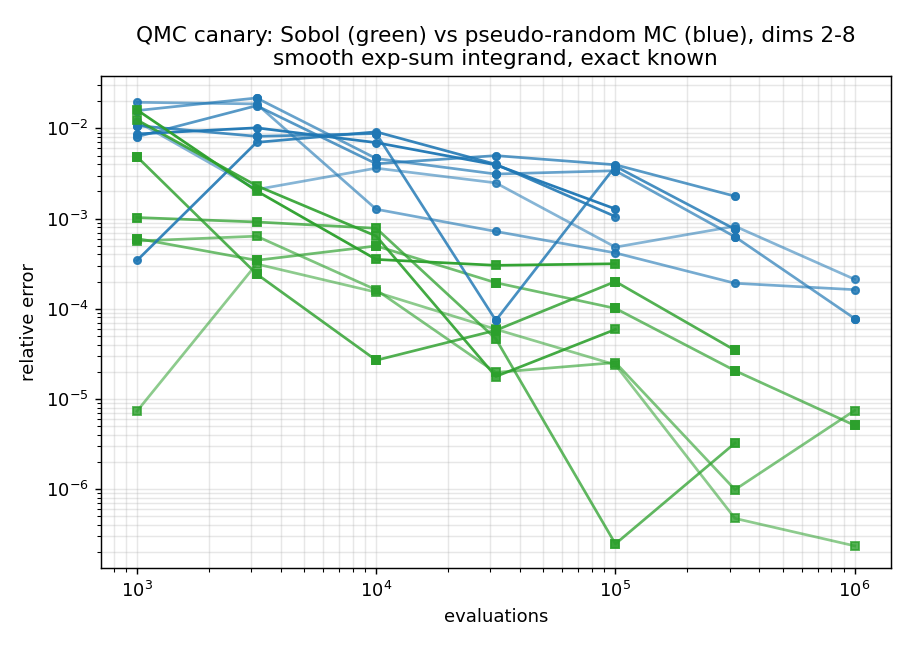
\includegraphics[width=0.62\textwidth]{canary.png}
\caption{QMC canary: Sobol (green) vs.\ pseudo-random MC (blue), dimensions
2--8, smooth exp-sum integrand.}
\end{figure}

%=============================================================================
\section{Results on the flattened sectors}

\subsection{Accuracy at the top budget}
Relative error vs.\ exact at the largest swept budget (bold = best in row).

\begin{center}\scriptsize
\setlength{\tabcolsep}{4pt}
\begin{tabular}{@{}lccccccc@{}}
\toprule
case & $n$ & MC & QMC & VEGAS & SUAVE & DIVONNE & CUHRE \\
\midrule
A\_simplex\_n2 & 2 & 6.8e\=4 & 8.2e\=6 & \best{2.0e\=6} & 7.8e\=4 & 8.9e\=6 & 3.9e\=5 \\
A\_simplex\_n3 & 3 & 1.5e\=3 & 6.9e\=5 & \best{1.6e\=6} & 3.5e\=4 & 1.9e\=5 & 2.8e\=5 \\
A\_simplex\_n4 & 4 & 9.4e\=4 & 4.2e\=4 & \best{2.0e\=6} & 4.5e\=4 & 1.8e\=4 & 4.4e\=4 \\
A\_simplex\_n5 & 5 & 4.3e\=3 & 1.1e\=3 & \best{8.5e\=5} & 4.7e\=4 & 1.3e\=2 & 1.6e\=3 \\
A\_simplex\_n6 & 6 & 8.9e\=4 & 1.8e\=3 & \best{1.6e\=4} & 9.3e\=4 & 1.1e\=2 & 2.4e\=2 \\
A\_simplex\_n7 & 7 & 1.8e\=2 & 1.7e\=2 & \best{4.4e\=4} & 3.0e\=3 & \warn{1.3e\=1} & 5.5e\=3 \\
A\_simplex\_n8 & 8 & 1.3e\=2 & 6.2e\=3 & \best{6.2e\=4} & 6.3e\=3 & \warn{2.2e\=1} & 4.9e\=3 \\
Af\_fracsimplex\_n2 & 2 & 6.9e\=4 & 9.3e\=6 & \best{1.4e\=6} & 2.2e\=4 & 6.3e\=6 & 1.6e\=5 \\
Af\_fracsimplex\_n4 & 4 & 9.2e\=4 & 9.4e\=5 & \best{5.7e\=6} & 5.0e\=4 & 7.1e\=5 & 2.9e\=4 \\
Af\_fracsimplex\_n6 & 6 & 6.2e\=3 & 5.2e\=3 & \best{1.2e\=4} & 4.4e\=4 & 2.6e\=3 & 3.9e\=3 \\
B\_quad\_n4 & 4 & 9.2e\=4 & 9.4e\=5 & \best{5.7e\=6} & 5.0e\=4 & 7.1e\=5 & 2.9e\=4 \\
B\_quad\_n6 & 6 & 6.2e\=3 & 5.2e\=3 & \best{1.2e\=4} & 4.4e\=4 & 2.9e\=3 & 3.9e\=3 \\
D\_product\_n3 & 3 & 4.1e\=4 & 6.9e\=6 & 1.1e\=5 & 8.2e\=4 & 2.7e\=5 & \best{2.1e\=7} \\
D\_product\_n4 & 4 & 2.5e\=4 & 1.8e\=5 & 6.0e\=6 & 1.3e\=4 & 9.8e\=5 & \best{3.1e\=6} \\
D\_product\_n5 & 5 & 5.2e\=4 & 5.8e\=5 & \best{3.3e\=7} & 6.4e\=4 & 3.9e\=3 & 9.0e\=7 \\
\bottomrule
\end{tabular}
\end{center}
Vegas is best or tied-best in 13/15 cases; Cuhre wins the two smooth product
cases.

\subsection{Empirical convergence rate $p$ \ ($\mathrm{rel.err}\sim N_{\rm eval}^{-p}$)}
\begin{center}\scriptsize
\setlength{\tabcolsep}{5pt}
\begin{tabular}{@{}lccccccc@{}}
\toprule
case & $n$ & MC & QMC & VEGAS & SUAVE & DIVONNE & CUHRE \\
\midrule
A\_simplex\_n2 & 2 & 0.28 & 0.80 & \best{1.07} & 0.07 & 0.29 & 0.03 \\
A\_simplex\_n4 & 4 & 0.42 & 0.66 & \best{1.40} & 0.59 & 0.61 & 0.18 \\
A\_simplex\_n6 & 6 & 0.80 & 0.35 & \best{1.21} & 0.91 & 0.43 & 0.05 \\
A\_simplex\_n8 & 8 & 0.22 & 0.63 & \best{1.56} & 0.85 & 0.21 & 0.30 \\
Af\_fracsimplex\_n4 & 4 & 0.47 & 0.86 & \best{1.15} & 0.37 & 0.50 & 0.23 \\
Af\_fracsimplex\_n6 & 6 & 0.47 & 0.61 & \best{1.06} & 0.81 & 0.15 & 0.45 \\
B\_quad\_n6 & 6 & 0.47 & 0.61 & \best{1.06} & 0.81 & \warn{$-0.09$} & 0.45 \\
D\_product\_n3 & 3 & 0.25 & 0.93 & 0.78 & 0.01 & 0.54 & 0.01$^\dagger$ \\
D\_product\_n5 & 5 & 0.35 & 0.62 & \best{1.73} & 0.23 & 0.44 & 0.08$^\dagger$ \\
\bottomrule
\end{tabular}
\end{center}
MC $\approx 1/\sqrt N$; QMC $\approx 0.6$--$0.9$ but eroding with $n$; VEGAS
$\approx 1.0$--$1.7$ and stable in $n$; CUHRE $\approx 0$ on A/Af/B (stalled),
while $^\dagger$on family~D it is already at $\sim\!10^{-7}$ from the smallest
budget (flat slope $=$ converged). DIVONNE is erratic, occasionally negative.

\begin{figure}[h]\centering
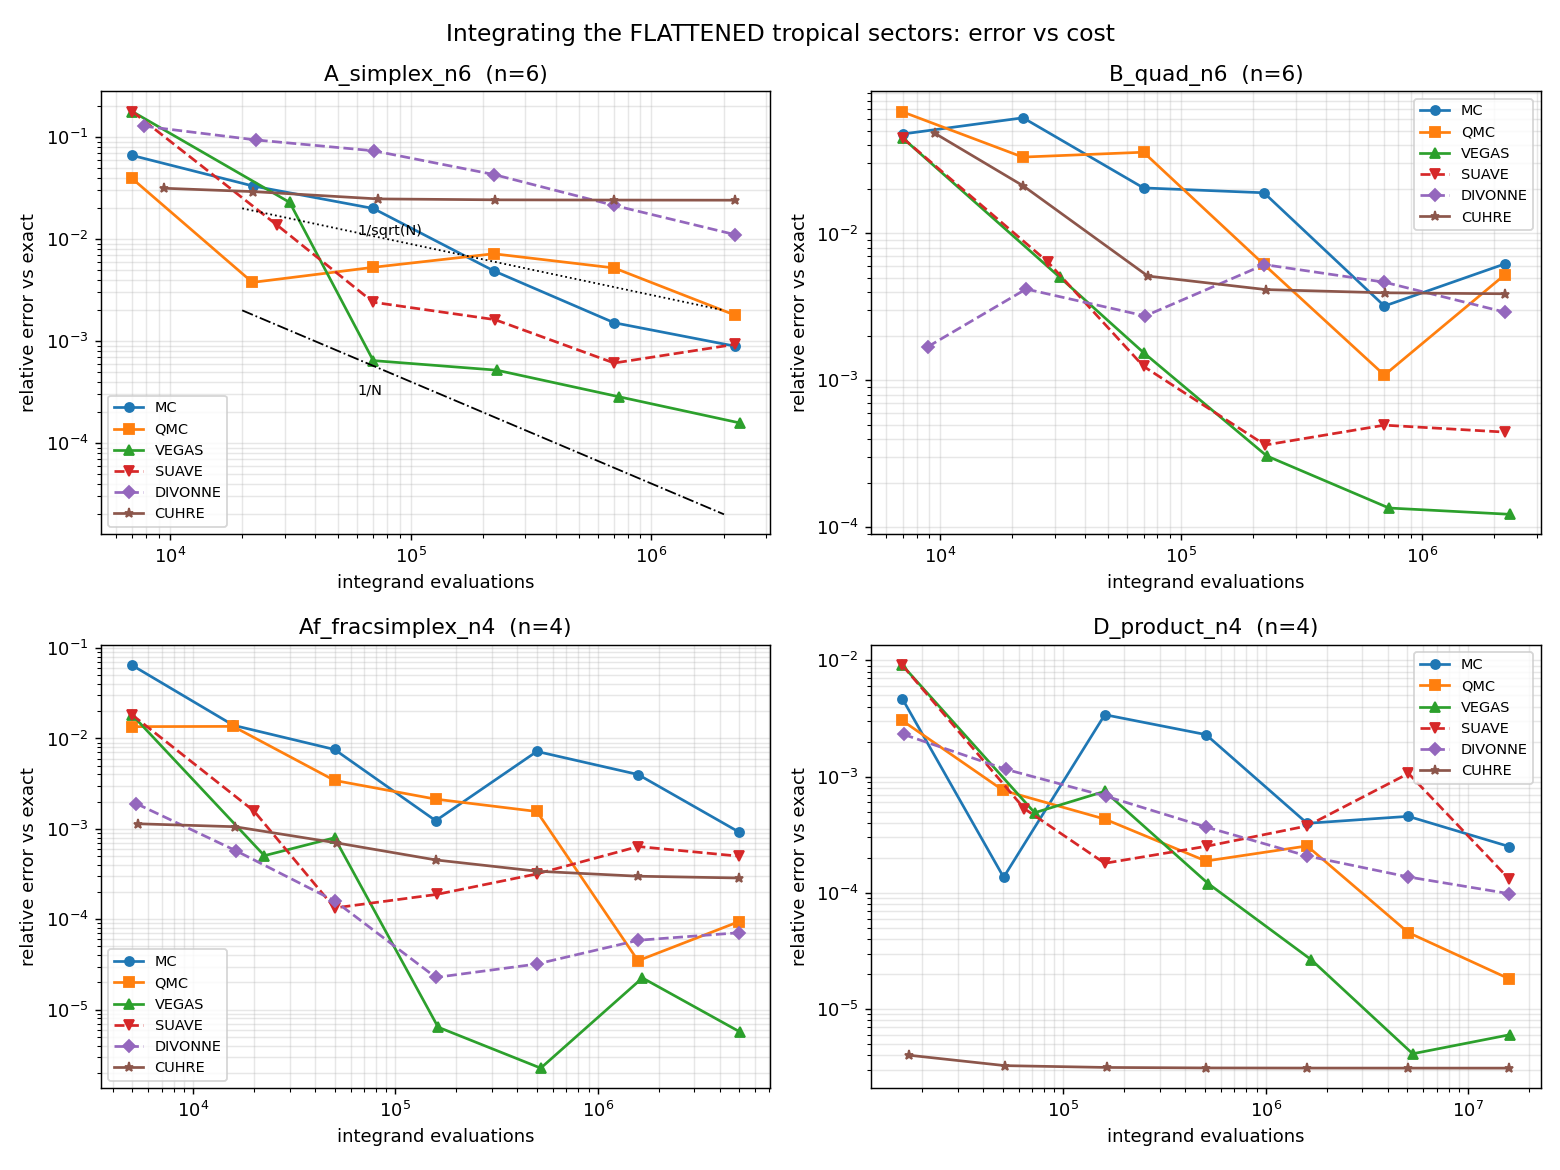
\includegraphics[width=\textwidth]{convergence.png}
\caption{Error vs.\ cost for four representative cases. Vegas (green) is lowest
with the steepest descent; Cuhre (brown) plunges to $\sim\!10^{-6}$ only for the
smooth product family (bottom right).}
\end{figure}

\subsection{Wall time to reach a target accuracy}
``Is it faster,'' made concrete. \dd{} $=$ not reached within the swept budget.

\begin{center}\scriptsize
\setlength{\tabcolsep}{5pt}
\textbf{Target: relative error $\le 10^{-3}$ (seconds)}\\[2pt]
\begin{tabular}{@{}lccccccc@{}}
\toprule
case & $n$ & MC & QMC & VEGAS & SUAVE & DIVONNE & CUHRE \\
\midrule
A\_simplex\_n3 & 3 & \dd & 0.021 & 0.004 & 0.018 & 0.009 & \best{0.002} \\
A\_simplex\_n4 & 4 & 1.600 & 0.018 & 0.025 & 0.024 & 0.271 & \best{0.003} \\
A\_simplex\_n5 & 5 & \dd & \dd & \best{0.005} & 0.007 & \dd & \dd \\
A\_simplex\_n6 & 6 & 0.181 & \dd & \best{0.006} & 0.095 & \dd & \dd \\
A\_simplex\_n7 & 7 & \dd & \dd & \best{0.025} & \dd & \dd & \dd \\
A\_simplex\_n8 & 8 & \dd & \dd & \best{0.151} & \dd & \dd & \dd \\
Af\_fracsimplex\_n6 & 6 & \dd & \dd & 0.102 & 0.130 & \best{0.011} & \dd \\
B\_quad\_n6 & 6 & \dd & \dd & \best{0.024} & 0.040 & \dd & \dd \\
D\_product\_n5 & 5 & 0.131 & 0.041 & 0.020 & 0.021 & \dd & \best{0.006} \\
\bottomrule
\end{tabular}
\end{center}
Vegas reaches $10^{-3}$ in all 15 cases and is the only method that survives to
$n=7,8$. At the tighter $10^{-4}$ target, Cuhre is fastest wherever the
integrand is smooth (product family, low-$n$ simplex), while Vegas is the most
broadly capable.

\subsection{Dimension scaling (simplex family, $10^5$ samples/sector)}
\begin{center}\small
\begin{tabular}{@{}rcccccc@{}}
\toprule
$n$ & MC & QMC & VEGAS & SUAVE & DIVONNE & CUHRE \\
\midrule
2 & \num{1.92e-4} & \num{1.19e-4} & \best{\num{1.15e-5}} & \num{3.78e-4} & \num{2.51e-5} & \num{3.86e-5} \\
3 & \num{1.05e-3} & \num{6.60e-4} & \best{\num{2.58e-5}} & \num{2.58e-4} & \num{7.14e-5} & \num{2.85e-5} \\
4 & \num{5.81e-3} & \num{3.51e-3} & \best{\num{2.39e-5}} & \num{1.61e-4} & \num{5.77e-4} & \num{4.47e-4} \\
5 & \num{2.19e-3} & \num{1.32e-3} & \best{\num{8.59e-5}} & \num{3.84e-4} & \num{2.14e-2} & \num{1.60e-3} \\
6 & \num{1.51e-3} & \num{5.21e-3} & \best{\num{2.85e-4}} & \num{6.09e-4} & \num{2.14e-2} & \num{2.41e-2} \\
7 & \num{1.84e-2} & \num{1.68e-2} & \best{\num{4.42e-4}} & \num{2.96e-3} & \warn{\num{1.33e-1}} & \num{5.47e-3} \\
8 & \num{1.28e-2} & \num{6.18e-3} & \best{\num{6.18e-4}} & \num{6.30e-3} & \warn{\num{2.20e-1}} & \num{4.93e-3} \\
\bottomrule
\end{tabular}
\end{center}
Wall times at this budget are within $\sim$2--3$\times$ across methods (Vegas
$\approx$ MC), so Vegas's 1--2 order-of-magnitude advantage is essentially free.

\begin{figure}[h]\centering
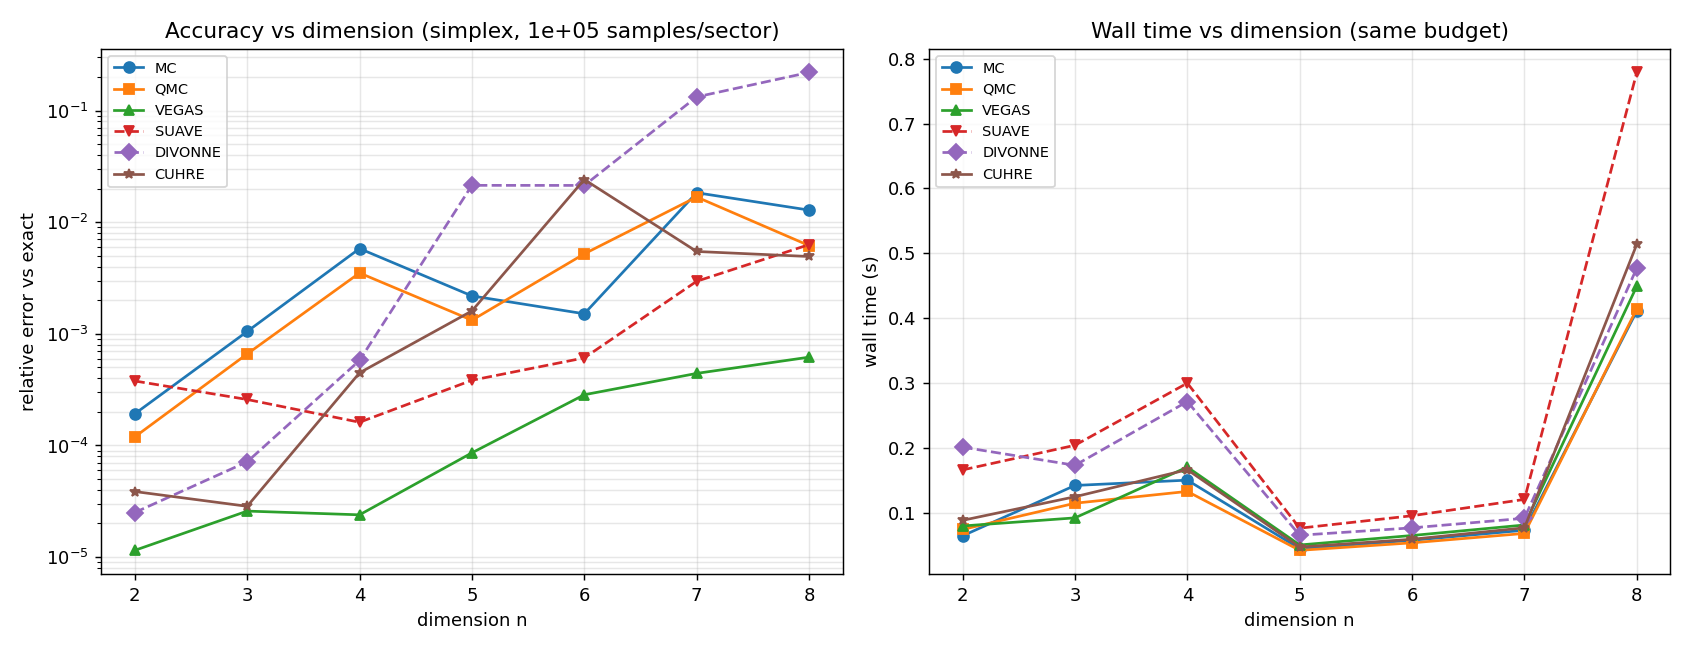
\includegraphics[width=\textwidth]{dimension_scaling.png}
\caption{Accuracy (left) and wall time (right) vs.\ dimension for the simplex
family. Vegas (green) stays $\sim$1--2 orders of magnitude ahead; Divonne
(purple) degrades to a $22\%$ error at $n=8$.}
\end{figure}

%=============================================================================
\section{Why Cuhre underperforms: flattening fixes magnitude, not smoothness}
Flattening uses $y=(y')^{1/a_{\mathrm{eff}}}$. Whenever a sector's effective
exponent $a_{\mathrm{eff}}\neq1$, this injects a fractional power at a cube
face. A real sector of \texttt{A\_simplex\_n4} ($a_{\mathrm{eff}}=2$) emits:

\begin{lstlisting}[language=C++]
// integrand_conv_2  (A_simplex_n4)
P0 += 1.0 * std::exp((1.0/2.0) * log_y[0]);   // == sqrt(y0)   <-- !
P0 += 1.0 * std::exp(1.0 * log_y[2]);
P0 += 1.0 * std::exp(0.0);
result *= std::exp(-6.0 * std::log(P0));
\end{lstlisting}

\noindent The integrand contains $\sqrt{y_0}$: value bounded (the $O(1)$ promise
holds), but \emph{first derivative infinite} as $y_0\to 0$. Polynomial cubature
(Cuhre, and Divonne's rule-based splitting) relies on bounded high derivatives
for both convergence and its error estimate, so it stalls. QMC (which wants
bounded Hardy--Krause variation) is partly hurt; plain MC is rate-agnostic;
Vegas's importance sampling reshapes the measure to absorb the edge and retains
the QMC rate. By contrast, every sector of the product family~D has all-integer
exponents ($a_{\mathrm{eff}}=1$):

\begin{lstlisting}[language=C++]
// integrand_conv_2  (D_product_n4)
P0 += 1.0 * std::exp(1.0*log_y[0] + 1.0*log_y[3]);   // smooth, rational
result *= std::exp(-2.0 * std::log(P0));
\end{lstlisting}

\noindent a $C^\infty$ rational integrand, on which Cuhre is unbeatable
($\sim\!10^{-7}$ in 6\,ms). \emph{On a flattened integrand, Cuhre's value is
decided by whether the flattening left it smooth --- i.e.\ whether the effective
exponents are integers --- which the standard decomposition does not control.}

%=============================================================================
\section{Verdict and recommendation}
\begin{center}\small
\begin{tabular}{@{}lp{10.5cm}@{}}
\toprule
method & verdict \\
\midrule
MC      & weakest; baseline only ($1/\sqrt N$, optimistic error bar on heavy sectors) \\
QMC (Sobol) & best no-dependency upgrade ($\sim$10$\times$ over MC); margin erodes with $n$ \\
\textbf{VEGAS} & \textbf{use this} --- best in every case, rate stable in $n$, cost $\approx$ MC \\
SUAVE   & acceptable but dominated by Vegas \\
DIVONNE & avoid --- erratic, can be silently/confidently wrong \\
CUHRE   & only for integer $a_{\mathrm{eff}}$ (smooth integrand) and modest $n$; then unbeatable \\
\bottomrule
\end{tabular}
\end{center}

\noindent\textbf{Recommendation.} Adopt CUBA-Vegas (Sobol, \texttt{seed=0}) as the
sector integrator; keep randomized Sobol QMC as the no-dependency fallback; use
Cuhre only when all effective exponents are integers and $n$ is modest; do not
use Divonne here. More broadly: \emph{smoothness, not magnitude, is the lever} ---
a flattening or lifting choice that yields integer effective exponents would
unlock deterministic cubature.

%=============================================================================
\section{Speed-up to reach the same accuracy}
Cost to hit a target relative error, as a factor over plain MC. Each method's
cost is the \emph{measured} smallest swept budget that crosses the target; MC is
extrapolated at its theoretical $1/\sqrt N$ from its largest-budget point
(\texttt{speedup.py}). Geometric mean across the 15 integrands (fewer
evaluations $=$ factor $>1$; wall-time is within ${\sim}5\%$ since per-evaluation
costs are similar):

\begin{center}\small
\begin{tabular}{@{}lccc@{}}
\toprule
target rel.\ error & QMC (Sobol) & \textbf{VEGAS} & Cuhre (smooth only) \\
\midrule
$10^{-3}$ & ${\sim}24\times$  & \best{${\sim}150\times$}  & $10^{2}$--$10^{3}\times$ \\
$10^{-4}$ & ${\sim}300\times$ & \best{${\sim}2300\times$} & $10^{4}$--$10^{5}\times$ \\
\bottomrule
\end{tabular}
\end{center}

\noindent Two points matter more than the headline figures. \textbf{(i) The
speed-up grows as the target tightens:} since Vegas converges like $N^{-1.3}$
vs.\ MC's $N^{-0.5}$, demanding $10\times$ more accuracy multiplies MC's cost
${\sim}100\times$ but Vegas's only ${\sim}6\times$ --- so Vegas climbs from
${\sim}150\times$ at $10^{-3}$ to ${\sim}2300\times$ at $10^{-4}$.
\textbf{(ii) At higher dimension the other methods do not reach the target at
all:} for $n\ge6$ at $10^{-3}$ (and $n\ge4$ at $10^{-4}$), MC/QMC/Suave/Cuhre
fail within a $10^5$--$10^6$/sector budget while Vegas succeeds --- there the
comparison is \emph{feasible vs.\ not}. Per-dimension Vegas eval speed-ups at
$10^{-3}$: $n{=}3{:}\,482\times$, $n{=}5{:}\,575\times$, $n{=}7{:}\,1038\times$,
$n{=}8{:}\,507\times$. Divonne is omitted from the headline because its
\emph{answers} can be wrong (\S3), so a fast route to a wrong value is moot.

%=============================================================================
\section{Is the tropical decomposition still worth it? (raw vs.\ flattened)}
The benchmark lives \emph{downstream} of the decomposition, so it is fair to ask
whether the decomposition still earns its keep once a good adaptive sampler is
used. I ran the package's \emph{raw-integrand} CUBA generator
(\texttt{cuba\_common.wl}, integrating the original integrand on
$[0,\infty)^n$ via $x_i=t_i/(1-t_i)$) with a \emph{generous} $2\times10^6$-eval
budget, against tropical+CUBA at a \emph{smaller} budget
(\texttt{raw\_vs\_tropical.wl}):

\begin{center}\small
\begin{tabular}{@{}llcc@{}}
\toprule
case & sampler & raw: rel.err @ neval & tropical+flattened: rel.err @ neval \\
\midrule
A\_simplex\_n6 & Vegas & \num{3.5e-3} @ 2.09M & \best{\num{2.8e-4} @ 0.73M} \\
Af\_fracsimplex\_n4 \ ($x^{-1/2}$) & Vegas & \num{7.7e-4} @ 2.09M & \best{\num{2.3e-6} @ 0.52M} \\
B\_quad\_n6 & Vegas & \num{3.1e-4} @ 2.09M & \best{\num{1.4e-4} @ 0.73M} \\
A\_simplex\_n6 & Cuhre & \best{\num{4.1e-4}} @ 2.0M & \num{2.4e-2} @ 0.70M \\
Af\_fracsimplex\_n4 \ ($x^{-1/2}$) & Cuhre & \num{3.4e-2} @ 2.0M & \best{\num{3.4e-4}} @ 0.50M \\
B\_quad\_n6 & Cuhre & \best{\num{1.2e-6}} @ 2.0M & \num{3.9e-3} @ 0.70M \\
\bottomrule
\end{tabular}
\end{center}

\noindent\textbf{Yes --- decisively, for the recommended sampler.} With Vegas
the flattened integrand is more accurate at fewer evaluations in every case, and
the gap is largest exactly where it should be: the $x^{-1/2}$ fractional simplex,
where the decomposition removes a genuine boundary singularity and is
${\sim}340\times$ more accurate using $4\times$ fewer evaluations than raw Vegas.
The decomposition is what \emph{creates} the tame $O(1)$ integrand the samplers
exploit; choosing the sampler is a second-order optimisation on top of it. (That
even plain MC reached ${\sim}10^{-3}$ in \S5 shows how much the decomposition
already did.)

The honest nuance is Cuhre-specific: when the \emph{raw} integrand is already
smooth (the simplex/quadratic with integer exponents), raw-Cuhre can beat the
flattened version, because flattening's $y=(y')^{1/a}$ substitution
\emph{introduces} the $\sqrt{\cdot}$ cube-edge derivative singularities of \S6.
But the moment the raw integral has a real singularity ($x^{-1/2}$), raw-Cuhre
collapses ($3.4\times10^{-2}$) and flattening wins (${\sim}100\times$). Flattening
thus trades a problem cubature can sometimes handle for one it cannot --- which is
fine, because the recommended method is Vegas, and the decomposition's real
payoff is on the structure that defeats every black-box sampler: integrable
singularities along coordinate hyperplanes, the non-compact domain, complex
oscillatory phases (flattening rotates the contour onto a log-spiral, manual
\S6.10), extreme coefficients (lifting), and the coefficient-blind fan --- one
symbolic preprocessing $+$ one compile serving \emph{thousands} of kinematic
points. The benign test integrands here understate this; real Feynman /
cosmological integrals are full of exactly that structure.

%=============================================================================
\section{Batch evaluation: one structure, 7200 coefficient sets}
The pipeline's headline use case is a \emph{kinematic scan}: the same polynomial
structure with many coefficient sets (the manual's example uses 7200). The fan
and flattened sectors are computed \emph{once}; the question is how to push 7200
coefficient sets through them. I built an explicit kinematic variant
(\texttt{gen\_kin.wl}, \texttt{bench\_batch.cpp}): $P=c_0+\sum_{i=1}^4 c_i x_i$,
$B=-6$, \texttt{KinematicSymbols}$=\{c_0..c_4\}$, exact
$I=1/(120\,c_0^2\prod c_i)$, 7200 coefficient sets, single-threaded.

Two facts dominate. \textbf{(1) CUBA \emph{does} batch via \texttt{ncomp}} --- a
vector-valued integrand with \texttt{ncomp}$=$\#points shares the sample
locations and adaptive refinement across all components in one call --- but there
is \emph{no native ``different parameters'' mode}, and this build caps
\texttt{ncomp} at \textbf{MAXCOMP$=1024$} (above it Cuhre returns \texttt{fail=-2}
and Vegas segfaults), so the 7200 points must be \textbf{chunked} into blocks of
$\le1024$. (\texttt{nvec} batches sample points for SIMD; \texttt{cubacores} adds
multicore --- orthogonal.) \textbf{(2) The biggest lever is sample-sharing}: in
the flattened integrand the costly transcendentals ($y'^{1/a}$, the monomial
basis $\exp(\sum e/a\cdot\log y)$, the prefactor) are
\emph{coefficient-independent}; only $\sum_m c_m\,\mathrm{basis}_m$ and one
\texttt{pow} differ per set. Computing the basis once per sample and reusing it
for all 7200 (\texttt{QMC\_shared\_basis}) is a pure win.

\begin{center}\small
\setlength{\tabcolsep}{6pt}
\begin{tabular}{@{}lcccc@{}}
\toprule
strategy & \multicolumn{2}{c}{M$=2000$} & \multicolumn{2}{c}{M$=8000$} \\
         & kp/s & rel.err & kp/s & rel.err \\
\midrule
MC per-kp \emph{(shipped)}       & 1{,}582 & 3.0e\=2 & 399 & 1.5e\=2 \\
QMC shared samples               & 2{,}188 & 1.9e\=2 & 546 & 9.4e\=3 \\
\textbf{QMC shared + shared-basis} & \best{6{,}617} & 1.9e\=2 & \best{1{,}654} & 9.4e\=3 \\
Vegas per-kp ($7200{\times}5$ calls) & 1{,}156 & 2.2e\=2 & 297 & \best{3.9e\=4} \\
Vegas \texttt{ncomp} (chunk $\le1024$) & 1{,}507 & 2.2e\=2 & 372 & 4.5e\=4 \\
\textbf{Cuhre \texttt{ncomp} (chunk $\le1024$)} & \best{1{,}721} & \best{1.7e\=3} & 478 & 5.9e\=4 \\
\bottomrule
\end{tabular}
\end{center}

\noindent\textbf{Findings.} \texttt{QMC\_shared\_basis} is the throughput champion
of the $\sim$1\%-accuracy tier --- ${\sim}4\times$ MC at \emph{identical} accuracy;
the basis-sharing amortisation applies to every method (I applied it only to QMC).
\texttt{ncomp}-batching beats per-kp CUBA (Vegas \texttt{ncomp} ${\approx}1.3\times$
faster than per-kp at equal accuracy: amortised sampling, 40 calls vs.\ 36{,}000);
per-kp CUBA is the \emph{wrong} way to batch. Batching partially \emph{reverses}
the single-integral verdict on Cuhre: pooling its many deterministic nodes across
a 1024-point chunk makes \texttt{Cuhre\_ncomp} both the most accurate and among the
fastest at moderate dimension ($n{=}4$ here: $1.7\times10^{-3}$ at 1{,}721 kp/s,
${\approx}18\times$ better than QMC) --- but its accuracy is set by the worst set in
a chunk and still degrades with dimension/non-smoothness, so this is
regime-specific. \textbf{Batch recommendation:} fast ${\sim}1\%$ scans $\to$ QMC with
shared samples $+$ shared basis (${\approx}4\times$ MC, trivially parallel over kp);
high accuracy at moderate $n$ $\to$ chunked \texttt{ncomp} Cuhre (ideally with the
shared-basis integrand); avoid per-kp CUBA. MC/QMC/per-kp-CUBA scale ${\sim}$linearly
over cores; \texttt{ncomp} CUBA parallelises over samples via \texttt{cubacores}.

\subsection{Dimension dependence: the same batch at $n=8$}
The $n{=}4$ result is \emph{not} representative at higher dimension. Re-running
the identical batch with $P=c_0+\sum_{i=1}^8 c_i x_i$ ($n{=}8$, 9 sectors)
\textbf{reverses the Cuhre finding}:

\begin{center}\small
\setlength{\tabcolsep}{6pt}
\begin{tabular}{@{}lccc@{}}
\toprule
strategy ($n{=}8$, M$=8000$) & kp/s & rel.err & (vs $n{=}4$) \\
\midrule
MC per-kp                       & 145 & 7.9e\=2 & 1.5e\=2 \\
QMC shared + basis              & \best{503} & 1.3e\=1 & 9.4e\=3 \\
Vegas per-kp                    & 106 & 5.1e\=2 & 3.9e\=4 \\
\textbf{Vegas \texttt{ncomp} ($\le512$)} & 128 & \best{5.0e\=2} & 4.5e\=4 \\
Cuhre \texttt{ncomp} ($\le512$) & 140 & \warn{9.5e\=2} & 5.9e\=4 \\
\bottomrule
\end{tabular}
\end{center}

\noindent Four things change. \textbf{(1)} 8D is intrinsically hard: the same
per-sector budget that gave ${\sim}1\%$ at $n{=}4$ gives only ${\sim}5$--$13\%$ at
$n{=}8$ ($\sim$100$\times$ more samples needed for ${\sim}1\%$), and heavy tails
worsen (MC max $>100\%$ on some sets). \textbf{(2)} \emph{Cuhre's batch win
evaporates} --- at $n{=}8$ it is \emph{worse than MC} (9.5e\=2 vs 7.9e\=2) and
slow: its deterministic rule needs many nodes per region in 8D (curse of
dimensionality), which batching cannot amortise away; ``chunked \texttt{ncomp}
Cuhre'' is for \emph{moderate} $n$ only. \textbf{(3)} Vegas is the only sampler
that still leads, \emph{given enough budget to adapt} (at a starvation budget
even Vegas trails MC; the single-integral study reaches $6\times10^{-4}$ at
$10^5$/sector while all else stalls); \texttt{ncomp} keeps its accuracy at
${\sim}1.2\times$ the per-kp throughput. \textbf{(4)} QMC's low-discrepancy edge
is gone --- a single-shift Sobol estimate is \emph{worse} than MC at $n{=}8$
(needs $N\gg2^n$); \texttt{QMC\_shared\_basis} stays the throughput champion but
only for rough scans. The safe \texttt{ncomp} chunk also shrinks with dimension
($1024$ crashes Vegas at $n{=}8$; use $\le512$).

\textbf{High-$n$ batch recommendation ($n\gtrsim6$--8):} budget ${\sim}100\times$
higher per sector; use \textbf{chunked-\texttt{ncomp} Vegas} as the accuracy
workhorse (the only rate that survives to 8D); \textbf{drop Cuhre}; keep
\texttt{QMC\_shared\_basis} only for fast rough scans; watch heavy-tail error
bars and lift extreme-coefficient sets.

\subsection{Wall-clock: a 7200-point $n=8$ scan on this machine}
Hardware: \textbf{Apple M2 Pro, 12-core (8 performance + 4 efficiency)}. Times
are for the single 8-D integral type above (9 sectors, 81 monomials, $P$
linear), single-threaded unless noted; accuracy is the \emph{median} over the
7200 sets and depends only on samples/sector $M$ (batch-size independent).

\begin{center}\small
\begin{tabular}{@{}lcc@{}}
\toprule
operating point & Vegas (chunked \texttt{ncomp}) & plain MC \\
\midrule
equal budget $M{=}8000$  & \best{4.98\% in 56 s} & 7.85\% in 50 s \\
equal budget $M{=}24000$ & ${\sim}0.5\%$ & 5.46\% in 270 s \\
\textbf{time to ${\sim}1\%$ median} & \best{${\sim}1.5$ min / ${\sim}10$--$15$ s (12 cores)} & ${\sim}1$--$2$ h / ${\sim}10$--$15$ min (12 cores) \\
\bottomrule
\end{tabular}
\end{center}

\noindent At \emph{equal} sample budget MC and Vegas cost about the same wall
time, but Vegas is ${\sim}10\times$ more accurate --- so to hit a fixed
${\sim}1\%$ target Vegas needs far fewer samples and finishes
\textbf{${\sim}30$--$60\times$ sooner}. On the 12-core M2 Pro a 1\%-accurate
7200-point $n{=}8$ scan is \textbf{${\sim}10$--$15$ s with Vegas vs
${\sim}10$--$15$ min with MC}. Caveats: \textbf{(i)} absolute seconds drift
$\pm1.5$--$2\times$ with the laptop's thermal state (the $M{=}24000$ MC run
clocked 270 s, ${\sim}1.8\times$ slower than a linear-in-$M$ extrapolation) --- the
MC/Vegas \emph{ratio} from one run is the robust quantity; \textbf{(ii)} MC's max
error across the sets was \textbf{421\%} (heavy tails, need lifting); Vegas held
its max to ${\sim}13$--$18\%$; \textbf{(iii)} QMC is no help at $n{=}8$ (worse than
MC: 7.25\% vs 5.46\% at $M{=}24000$); \textbf{(iv)} both columns scale
${\sim}$linearly with $\#\text{sectors}\times\#\text{monomials}$ (the ratio holds);
one-time preprocessing is seconds-to-a-minute, separate.

%=============================================================================
\section{Limitations}
Single-threaded; budgets capped at $10^5$--$10^6$ samples/sector (enough to fix
the ranking and rates, not tuned to a fixed high-precision target; MC/QMC
parallelize trivially over kinematic points as the shipped code does).
Convergence slopes are finite-range least-squares fits; for adaptive routines
(Vegas) an apparent $p>1$ reflects grid lock-on and should be read as ``much
faster than MC,'' not a literal asymptotic exponent. A thin-lattice-simplex
workaround was required: the packaged fan code needs an integer interior point,
which \texttt{conv}$\{0,e_i\}$ lacks for $n\ge4$; since the normal fan is
scale-invariant the fan is computed from \texttt{conv}$\{0,(n{+}2)e_i\}$
(validated against direct \texttt{NIntegrate}). All four CUBA routines and Sobol
QMC agree with the exact reference (except Divonne), so the conclusions are not
artifacts of one implementation.

\paragraph{Environment.} macOS / Apple silicon; Apple clang 14
(\texttt{-std=c++17 -O3}); CUBA 4.2.2 and Boost 1.90 (Homebrew); Polymake 4.15;
Wolfram Engine. Data: \texttt{TEST/INTERFILES/results.csv} (769 rows).
Reproduce: \texttt{gen\_sectors.wl $\to$ run.sh $\to$ analyze.py $\to$ plots.py}.

\end{document}
